\documentclass[oneside]{book}
\usepackage[a4paper,top=2.5cm,bottom=2.5cm,left=2.5cm,right=2.5cm]{geometry}
\usepackage[utf8]{inputenc}
\usepackage{makeidx}
\usepackage{graphicx}
\usepackage{multicol}
\usepackage{float}
\usepackage{listings}
\usepackage{color}
\usepackage{ifthen}
\usepackage[table]{xcolor}
\usepackage{textcomp}
\usepackage{alltt}
\usepackage{amsmath}
\usepackage[scaled=.90]{helvet}
\usepackage{courier}
\usepackage{sectsty}
\usepackage{hyperref}
\usepackage[titles]{tocloft}
\usepackage{wrapfig}
\lstset{language=C++,inputencoding=utf8,basicstyle=\footnotesize,breaklines=true,breakatwhitespace=true,tabsize=8,numbers=left }
\makeindex
\setcounter{tocdepth}{3}
\hfuzz=15pt
\setlength{\emergencystretch}{15pt}
\hbadness=750
\tolerance=750

\begin{document}
\begin{titlepage}
\vspace*{7cm}
\begin{center}
{\Huge wxChaos \\[1ex]\large 1.\-2.\-0 }\\
\vspace*{1cm}
{\large User manual}\\
\vspace*{0.5cm}
\end{center}
\end{titlepage}
\pagenumbering{roman}
\tableofcontents
\pagenumbering{arabic}
\chapter{Introduction}
\textit{wxChaos} is a fractal generating program whose main purpose is to provide the user the capability to explore the world of the fractal geometry, and also provide an interface to create new fractal using formulas or a scripting language. The intention is to provide a tool to learn what are fractals, how to draw them and give the user the capability to create them.

There are a lot of programs in the internet to draw fractals, programs that are also open source. Before that we may ask, what does \textit{wxChaos} has to offer? One of the features is the great number of fractals pre-implemented. Other feature is the inclusion of a scripting language, so the user can learn to program them.

\textit{wxChaos} is a free tool that is distributed under a open source license, which means that any person can inspect, use, and modify the source code. For more information check the license chapter.

\chapter{What is a fractal?}
From MathWorld:
\quote{“A fractal is an object or quantity that displays self-similarity, in a somewhat technical sense, on all scales. The object need not exhibit exactly the same structure at all scales, but the same "type" of structures must appear on all scales.”}

A simple and illustrative example of fractal is the Sierpinsky triangle, which is constructed making division on a triangle.
\begin{figure}[h!]
	\centering
	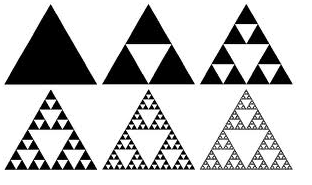
\includegraphics[scale=0.7]{img/triangle.png}
	\caption{Sierpinsky triangle}
	\label{triangle}
\end{figure}

Doing this procedure infinite times makes a fractal, this is seen by doing a zoom in the image and seeing that the zoomed image has the same form of the original triangle, meaning that is auto-similar. The same procedure is valid with squares, lines and other types of figures.

\begin{figure}[h!]
	\centering
	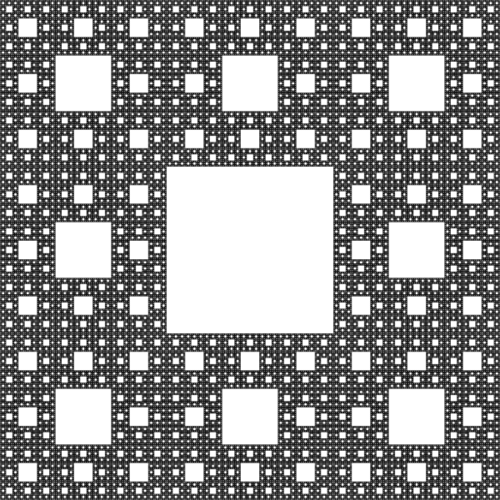
\includegraphics[scale=0.25]{img/carpet.png}
	\caption{Sierpinsky carpet}
	\label{carpet}
\end{figure}

Analysing the object it can be verified a paradoxic fact: The object doesn't have any area! And yet is an object that is represented in a bi-dimensional plane (like your computer screen). It is said that the object doesn't have any area because it you would make a infinite number of divisions in the triangle there wouldn't be any area left. Now imagine that you take the Sierpinsky triangle and grab it by the sides and stretch it. It would happen something even odder: It's length would be infinite.

The reason for this lies in the fact that a fractal doesn't necessarily has integer dimensions like the ones that we know (1 dimension for lines, 2 dimensions for areas and 3 form volumes), fractals can have fractional dimensions. For example, the Sierpinsky triangle has a dimension of $1.58496$, and that is the reason of why you can't describe the triangle on terms of area (has less that 2 dimensions), but also can't be described in terms of longitude (has more than 1 dimension). This number is known as \textit{fractal dimension}.

It's because the same fact that you can make infinite zooms over fractals and still see a variety of auto-similar figures.

Another type of fractals that are more interesting are the ones made by plotting a series of numbers in the complex plane. These show a more rich variety of figures and forms, and these are the ones that \textit{wxChaos} plots. Examples of fractals plotted in the complex plane are the Mandelbrot set and the Julia set.

\chapter{Program GUI}
The program has a simple user interface whose main purpose is to clearly show the rendering area. In the upper left corner the number of iterations is shown. You could think of the iterations as the number of steps that the program does to render the fractal. In the previous example with the Sierpinsky triangle each time that the triangle was divided and iteration was being made. In this case an iterations refers to a math operations with the fractal formula. On more iterations the final image will have better quality but it will take more time to render it. Another thing that may also affect performance is the window size. On a bigger window the program will need to perform more operations, so it will be slower.

\begin{figure}[h!]
	\centering
	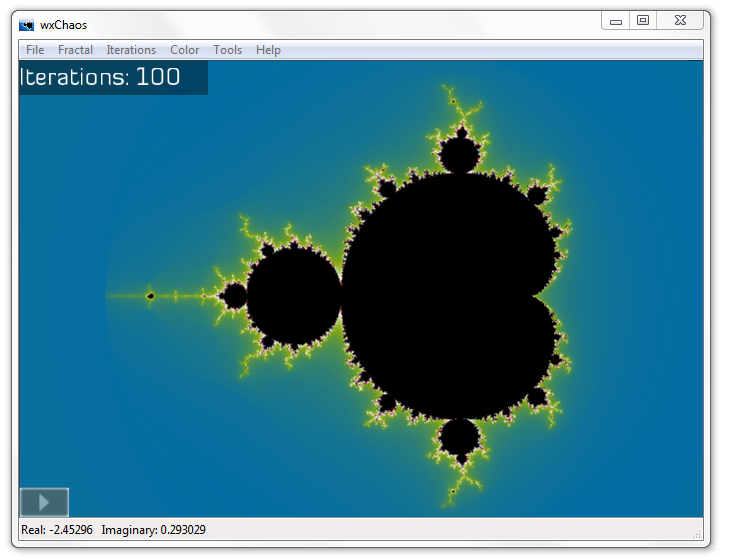
\includegraphics[scale=0.5]{img/sc1.png}
	\caption{User interface}
	\label{GUI}
\end{figure}

In the lower part of the main window two labels are shown: \textit{real} and \textit{imaginary}. These labels refer to the position of the cursor inside of the fractal plane (that may be complex or Cartesian, depending on the fractal). In the case of a complex fractal it's horizontal axis is called the \textit{real axis} and the vertical axis is called \textit{imaginary axis}. 

To perform a zoom over the image it only takes a click to begin selecting a rectangle that will be the new zooming area. To zoom back use a right click.
Next, the elements of the menu will be described.


\subsection{Fractal}
\begin{description}
\item[Formula] Each fractal is described by a characteristic formula to render it. In this menu the user can select different formulas that render fractal with different forms.

\item[Enter Julia constant] Some fractals of the Julia variety depend of a number that is the $k$ constant. In this element some options are provided to change this constant. The manual method is useful when is required to introduce a number with precision. The slider is to have a quick view of how the fractal changes when the constant is also changed. The slider works taking the $k$ constant from the point that is targeted inside the complex plane in the fractal rendering area.

\item[Julia mode] Some fractal of the Mandelbrot variety like Mandelbrot $z = z^2 + c$, Mandelbrot $z = z^n + c$, Manowar and Burning Ship have the option to create a window with it's Julia variant. The slider enables the user to select the $k$ constant.

\item[Show orbit] This options allows to visualize the orbit that the selected point performs when iterated. The orbit will have a red color if it diverges, and a red color if converges to some value.

\item[Enter user formula] Allows the user to introduce it's own formulas.

\begin{figure}[h!]
	\centering
	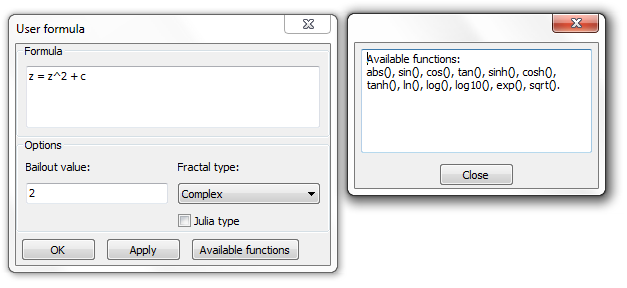
\includegraphics[scale=0.5]{img/sc6.png}
	\caption{User formula}
	\label{GUI}
\end{figure}

The user formulas allows the user to create two types of fractals: Complex fractals and fractals created using a numerical method known as \textit{fixed point method}. The \textit{bailout} refers to the position that the point must acquire in the orbit to decide if the point belongs to the fractal set (and paint it black). This menu also allows to select if the fractal will be of the Julia variety. The formulas must be written using the variables $z$, $c$ or $Z$ and $C$. In the case that there is an error in the formula this will be described in the console.

\item[Fractal options] Some fractals have optional parameters that may be changed in this panel.
\end{description}

\subsection{Iterations}

\begin{description}
\item[Manual iterations] Allows the user to manually establish the number of iterations.
\item[Increase iterations] Increases a predefined number of iterations. The standard number are $20$ iterations, but some fractals like \textit{Double pendulum} may change more iterations.
\item[Decrease iterations] Decreases a predefined number of iterations.
\end{description}

\subsection{Color options}
When the fractal is rendered it doesn't have any specific information on how it must render the colors. It actually has to use an algorithm to interpret which color should be used.

\textit{wxChaos} uses two methods to create the color palette. The standard way is using a color gradient. In this menu the user may select the colors to create a custom gradient. Another way to generate a color palette is to use the \textit{STD color}, that is also capable of creating interesting results.

To use the color palettes the fractal needs an algorithm to assign these colors first. The available algorithms will be shown.

\begin{description}
\item[Escape time] The escape time algorithm is the most basic of all, and no doubt that is the fastest available in the program. This algorithm measures how many iterations have passed to determine if the point belongs to the fractal set. If it belongs to the fractal set paints the point black, if not assigns a color depending of the number of iterations. You may notice the discontinuous color lines, in artistic terms this is a defect of the algorithm, but it may be corrected with the \textit{smooth render option}, which reduces this effect. Another option is the orbit trap. This one measures how close did the iterated point got to some point or line, called the orbit trap, and colors according to that.

\begin{figure}[h!]
	\centering
	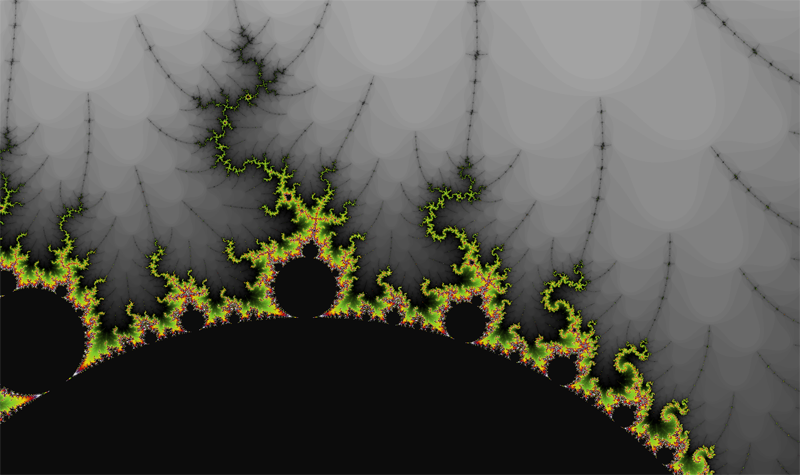
\includegraphics[scale=0.3]{img/fractal0.png}
	\caption{Escape time algorithm}
	\label{Escapetime}
\end{figure}

\begin{figure}[h!]
	\centering
	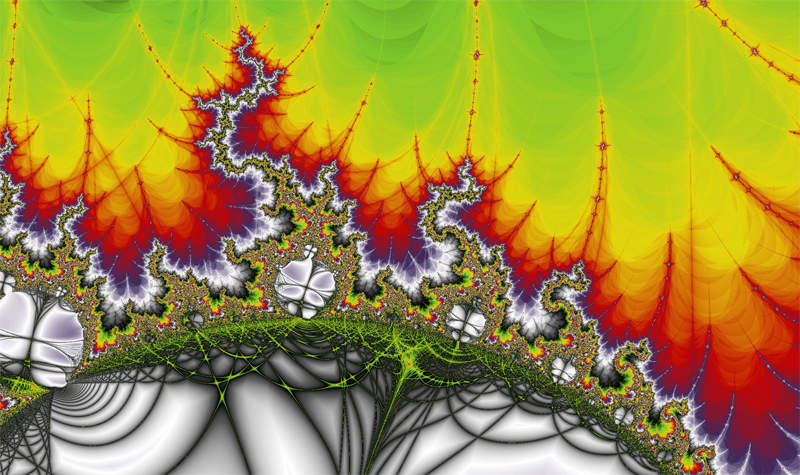
\includegraphics[scale=0.3]{img/fractal3.png}
	\caption{Escape time algorithm with orbit traps}
	\label{Orbit trap}
\end{figure}

\item[Gaussian integer] The Gaussian integers are integers inside the complex plane, numbers which real and imaginary part are integers. This algorithm is also an orbit trap, but it's distributed along the complex plane. This algorithm produces better results with relative colors.

\begin{figure}[h!]
	\centering
	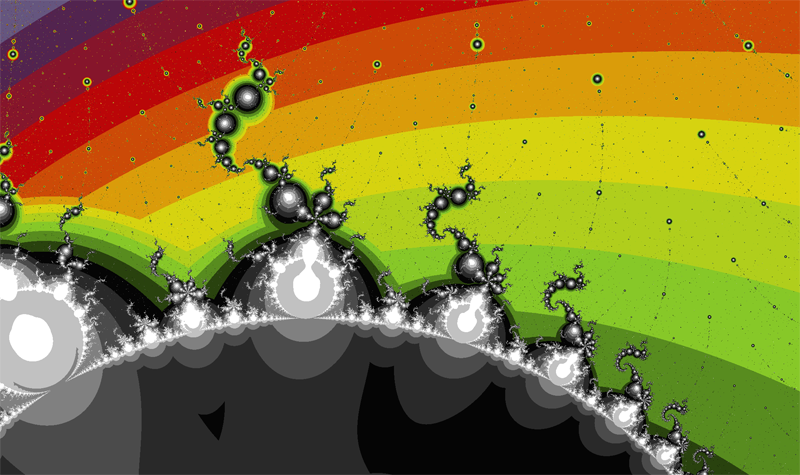
\includegraphics[scale=0.3]{img/fractal4.png}
	\caption{Gaussian integers algorithm}
	\label{GaussianInt}
\end{figure}

\item[Buddhabrot] This algorithm throws random points to the visible section of the complex plane and iterates them. Each point marks it's position in every iteration, and the final result is shown on the screen.

\begin{figure}[h!]
	\centering
	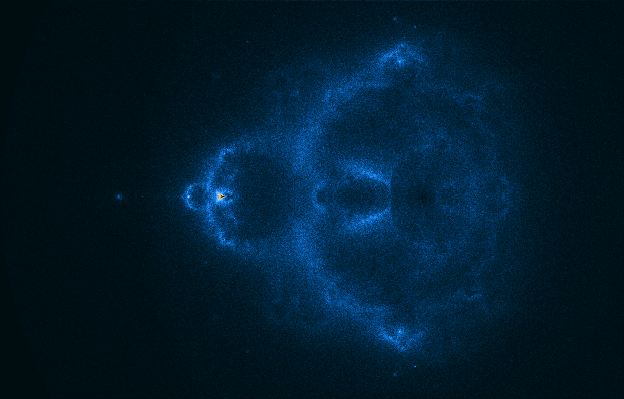
\includegraphics[scale=0.4]{img/fractal6.png}
	\caption{Buddhabrot}
	\label{Buddhabrot}
\end{figure}

\item[Escape angle] The escape angle algorithm is very similar to the scape time algorithm, but instead of measuring the the number of iterations, it measures the final position of the iterated point. T.

\begin{figure}[h!]
	\centering
	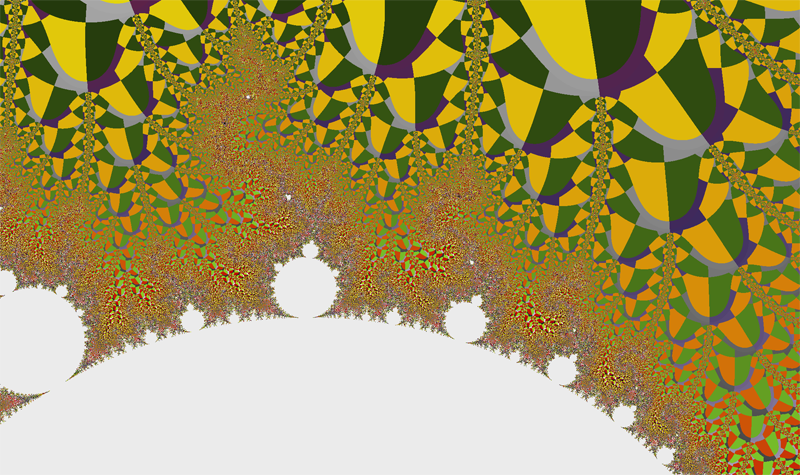
\includegraphics[scale=0.3]{img/fractal5.png}
	\caption{Escape angle}
	\label{escapeAngle}
\end{figure}

\item[Triangle inequality] This algorithm is based on a euclidean geometry theorem known as \textit{triangle inequality}. This algorithm gets better results using relative colors.

\begin{figure}[h!]
	\centering
	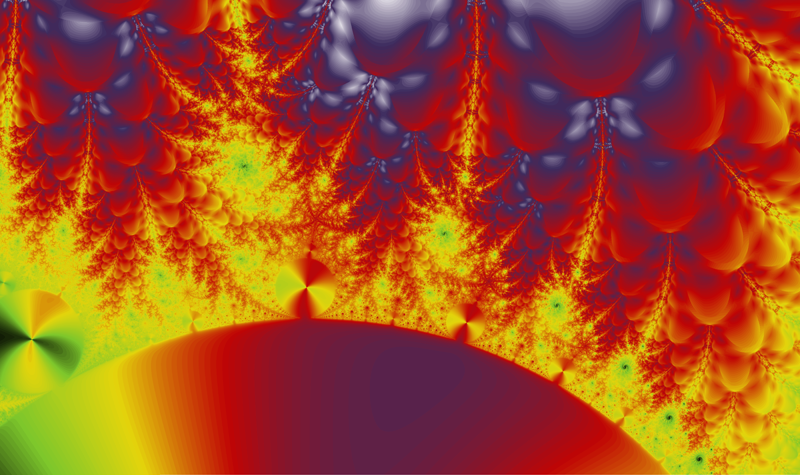
\includegraphics[scale=0.3]{img/fractal1.png}
	\caption{Triangle inequality}
	\label{Triangle}
\end{figure}

\end{description}

\subsection{Gradient}
The gradient is a color progression made from various colors in different positions. To obtain better results it's recommended that the first and the last color coincide.

\subsection{Gaussian Color}
The Gaussian Color algorithm generates a color palette from a normal distribution. To every number of iterations a color that is the sum of the normal distribution in each channel is assigned. In the panel the user may modify the intensity (coefficient), the position (mean of the distribution) and it's standard deviation.

\begin{figure}[h!]
	\centering
	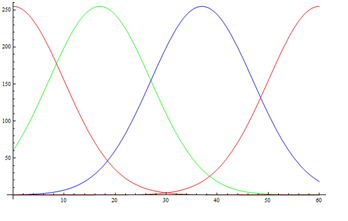
\includegraphics[scale=0.8]{img/dist.png}
	\caption{Color distribution}
	\label{Color dist}
\end{figure}

This type of coloring is not as easy to configure as the gradient, so it's not always recommended.

\chapter{User fractal}

Another of the capabilities of \textit{wxChaos} is that lets the user introduce custom formulas. The user formulas may be a complex series or fractals created from the numerical method known as the \textit{fixed point method}. To delve into this section a minimum math knowledge is required.

\subsection{Complex numbers}
Before beginning to render fractals it's necessary to define first the concept of a complex number. Complex numbers are an extension of the concept of number, giving this number a real part and a imaginary part. It suffices to say that all the arithmetic operations like sum, rest, multiplication and division are defined for this complex numbers. A way to represent this complex numbers is visualizing the real part as a horizontal axis of the number and the imaginary part as a vertical axis, so now the complex number can be represented on a plane. This plane it's called the \textit{Argand} plane.

\begin{figure}[h!]
	\centering
	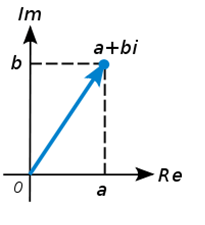
\includegraphics[scale=0.7]{img/complex.png}
	\caption{Argand plane}
	\label{Argand}
\end{figure}

This \textit{Argand} plane is the area shown when rendering a fractal.

\subsection{Rendering fractals}
Mathematically speaking when a fractal is rendered we are making a series of complex numbers, and we are only checking the convergence of this series before an initial condition. So, what does it mean to have a formula like $Z_{n+1} = Z_n^2 + C$ (Mandelbrot set)? When a fractal is rendered we are traveling through each pixel in the screen taking the corresponding coordinates of the Argand plane. This point will be the $C$ constant. Then we will iterate this point from the Mandelbrot formula.

\[
	Z_0 = C
\]
\[
	Z_1 = C^2 + C
\]
\[
	Z_2 = (C^2 + C)^2 + C
\]
\[
	Z_3 = ((C^2 + C)^2 + C)^2 + C
\]
\[
	Z_4 = (((C^2 + C)^2 + C)^2 + C)^2 + C
\]

Following this procedure during $N$ iterations and after performing the bailout check it will be determined if the series converge or diverge. This will be done to every pixel on the screen. If the value of the norm of $Z$ is greater than the bailout then that will mean that the series diverge so the pixel will be painted with some color (depending on the algorithm), if it's minor it will converge so the pixel will be painted black, which means that the point belongs to the set given by the formula. 

To better appreciate this \textit{wxChaos} has the \textit{show orbit} mode.

\begin{figure}[h!]
	\centering
	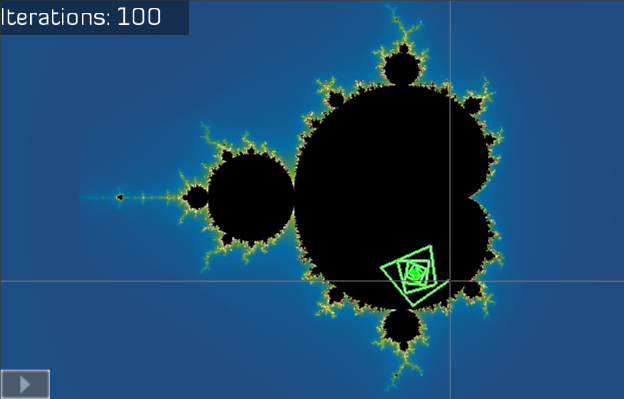
\includegraphics[scale=0.7]{img/sc7.png}
	\caption{Convergent orbit}
	\label{Orbit1}
\end{figure}

\begin{figure}[h!]
	\centering
	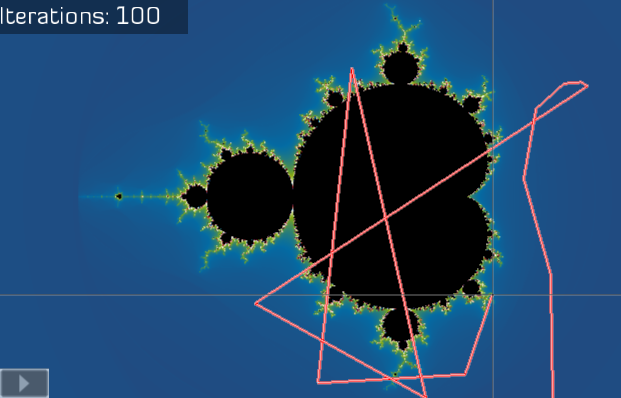
\includegraphics[scale=0.7]{img/sc8.png}
	\caption{Divergent orbit}
	\label{Orbit2}
\end{figure}

This mode allows the user to select a point in the complex plane and see it's orbit when iterated. The orbit will be green if the orbit converges and red if it diverges.

The fractals rendered with the fixed point method differ in the rendering method. These are based in the numerical method called \textit{fixed point method}, which has the amazing feature that it's convergence it's chaotic. This type of fractals measure the position of the last iterated point to determine the color. The optional parameter of these fractals, \textit{min step} is the minimum amount of movement that must have the point to determine that has arrived to the solution.

\subsection{Numerical methods}
Now I will explain what are the numerical methods and how you can render fractal with them.
When we are solving a equation we know (or we should know) how to find it's solutions with elemental algebraic procedures. To a human this is relatively easy. But giving the same capabilities to a computer it's not a easy task. This is the reason why the numerical methods are so popular. The numerical methods use an algorithm to successively approximate to the solution of a equation, and it doesn't involve doing algebra which is a great advantage. Examples of numerical methods are the \textit{Newton-Rhapson method}, the \textit{fixed point method}, the \textit{secant method}, the \textit{bisection method}, etc. The surprising thing is that if you apply some of these methods to solve a complex equation, they exhibit chaotic behavior! So they are ideal to render fractals from them.

To make a fractal from a numerical method what it's done is to take all the points in the \textit{Argand} plane as initial conditions, and then the numerical method is applied so the point converges to one solution. At last the point is colored depending to which solution converged.

\chapter{Tools}
\textit{wxChaos} comes with some tools to explore characteristics of the fractals.

\subsection{Dimension Calculator}
A very interesting thing on fractals is that they do not have an integer dimension like the classical geometric shapes. You know, the line has 1 dimension, the square 2, and the cube is three dimensional. With fractals you cant apply the same rule. Why is that? With regular geometric shapes like an square if you measure the area and then measure it again with an smaller ruler there is no change on the result. It doesn't matter the scale of the measuring device, it will always yield the same results. With fractals it's all backwards! Depending on the size of the ruler you will have different results.

\begin{figure}[h!]
	\centering
	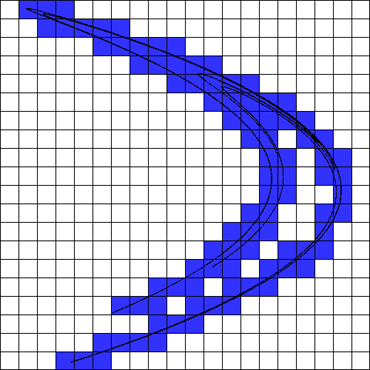
\includegraphics[scale=0.4]{img/dim.png}
	\caption{Box counting}
	\label{Dimension}
\end{figure}

Now, the formal way to do this is to divide the image in multiple sections (boxes) and count how many boxes are depending on the size of the boxes. The relationship between the number of boxes and the size of the boxes will give you the fractal dimension. More exactly the Minkowski-Bouligand dimension (there are many definitions of fractal dimension).

\begin{figure}[h!]
	\centering
	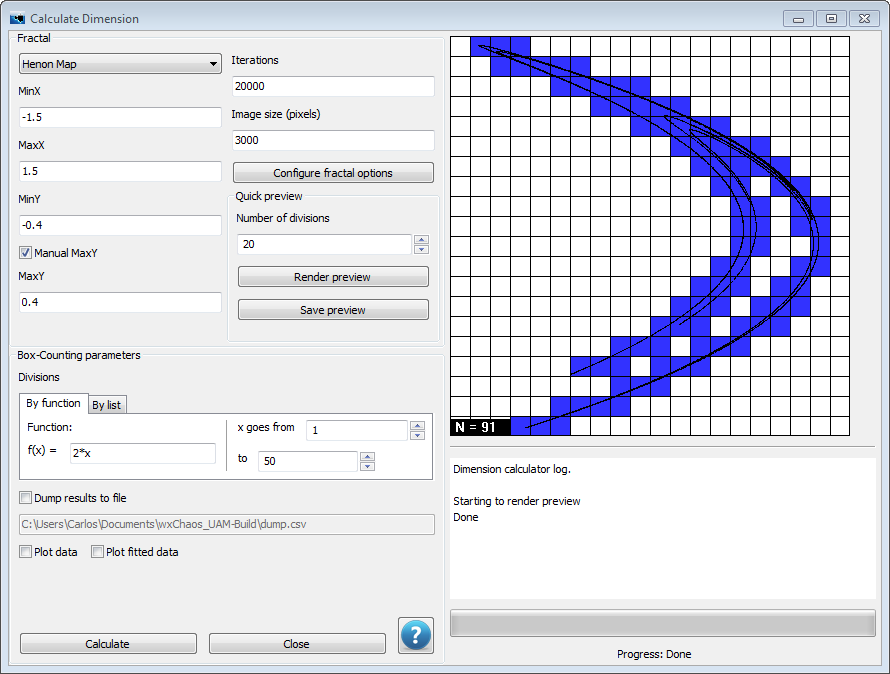
\includegraphics[scale=0.4]{img/sc9.png}
	\caption{Dimension calculator dialog}
	\label{Dim dialog}
\end{figure}

Let's call the size of the box by epsilon. To have more accurate results you need many points to perform a calculation. You can adjust this on the box counting parameters. The first way to select the points (sizes of epsilon) is to generate them by a function. For example if the function is $f(x) = 2x$ and x goes from 1 to 4 your epsilon sizes would be 2, 4, 6, 8. You can also select the sizes by list. Just write them manually.

You can also plot the results of the calculation. When all the points have been counted, the program will calculate the dimension using the following formula:

\[
	\dim_{\rm box}(S) := \lim_{\varepsilon \to 0} \frac {\log N(\varepsilon)}{\log (1/\varepsilon)}
\]

The fitted data plot it's just a logarithmic plot, useful to see the convergence.

\subsection{Script editor}
\textit{wxChaos} comes with an script editor and its debugger to create custom fractals. In the current version the debugging features are limited to syntax check and a previsualization of the resulting image. For more information about the scripting API check the chapter \ref{chap:scripts}.

\subsection{Zoom recorder}
This tool enables the user to record a video zoom. To use it, first perform a zoom in the main fractal visualizer and then open the zoom recorder. You can preview the route and configure parameters like speed and color rotation in the menu. Note: The zoom recorder will not work if the user has not performed any zoom in the visualizer.

\chapter{User scripts}
\label{chap:scripts}

\textit{wxChaos} gives the user the capability to creates it's own fractal through scripts. The scripts are created in a language very similar to C++ called \textit{Angelscript}. It suffice to have basic notions of C++ to create a fractal with no difficulty.

The user scripts will be saved in the \textit{UserScripts} folder. The program will load the existing scripts automatically when executed, and the scripts will be available in the formula menu. The scripts shown in this manual can be found inside the \textit{ScriptSamples} folder. You only need to copy them to the \textit{UserScripts} folder to execute them.

The program makes use of the console to communicate the user any error during the compilation or execution of the script. Also the script may send messages to the console. This is useful when debugging the script.

\subsection{Hello fractal world}
When learning a new programming language the first exercise usually is the \textit{hello world} program, whose only purpose is to show the "Hello world" words on the screen. This is to show the general structure of the language. To those used to C/C++ the \textit{Hello fractal world} presents some differences respect to the C/C++ analogue. To begin with in C/C++ there is a entry point; the \textit{main} function. In the case of \textit{Hello fractal world} there are two entry points. One is the \textbf{Configure} function which is used to establish the fractal options and the information that will be shown on the menu, and the other entry point is the \textbf{Render} function. This is the one that renders the fractal onto the screen. In this \textit{Hello fractal world} we won't draw any fractal on the screen, we will simply send some text to the console.

\begin{lstlisting}
void Configure()
{
	SetFractalName("Hello world");
	SetCategory("Other");
}

void Render()
{
	if(threadIndex == 0)
	{
		PrintString("Hello fractal world\n");
		PrintInt(34);
		PrintString("\n");
		PrintFloat(0.02);
		PrintString("\n");
		complex z(0.23, 389);
		PrintComplex(z);
	}
}
\end{lstlisting}

When executing the script it produces the following output:
\begin{lstlisting}
Hello fractal world
34
0.02
0.23+i389
\end{lstlisting}

Notice that unlike C/C++ it wasn't necessary to include any header. This is because all the necessary functions and variables are defined inside \textit{wxChaos}.

\subsection{Script functions and variables}
A description of all the variables and functions available inside the scripts will be presented.

\textbf{Functions:}
\begin{description}
\item[SetFractalName(string)] Sets the name of the fractal.
\item[SetCategory(string)] Sets the fractal category. Available: \textit{Complex, NumMet, Physic, Other}.
\item[SetMinX(float)] Set left limit.
\item[SetMaxX(float)] Set right limit.
\item[SetMinY(float)] Set lower limit.
\item[SetJuliaVariety(bool)] Specifies if the fractals is a Julia variety.
\item[SetDefaultIter(int)] Sets the default iteration number.
\item[SetRedrawAlways(bool)] Set this to \textbf{true} if you need to redraw all the fractal every time the user moves the view position.
\item[NoSetMap(bool)] Set this to \textbf{true} if your fractal doesn't make use of the set map. This prevent it from appearing in the dimension calculator.
\item[PrintString(string)] Sends text to the console.
\item[PrintInt(int)] Prints a integer on the console.
\item[PrintFloat(float)] Prints a real number (float) on the console.
\item[PrintComplex(complex)] Prints a complex number on the console.
\item[SetPoint(int x, int y, bool inSet, int iter)] Set point in the  $(x,y)$ coordinates of the plane. The parameter \textbf{inSet} is used to determine if the point belongs to the set. If \textit{true} it will be painted black. I \textit{false} it wont be painted, instead a color will be picked from \textbf{iter}, that is the number of iterations that were used to determine if the point belonged to the set.
\end{description}

\textbf{Variables:}
\begin{description}
\item[minX] Selected left limit.
\item[maxX] Selected right limit.
\item[minY] Selected lower limit.
\item[maxY] Upper limit.
\item[xFactor] Conversion factor screenWidth -> horizontal axis.
\item[yFactor] Conversion factor screenHeight -> Vertical axis.
\item[kReal] K Real constant in Julia mode.
\item[kImaginary] K Imaginary constant in Julia mode.
\item[ho] Upper limit in thread section.
\item[hf] Lower limit in thread section.
\item[wo] Left limit in thread section.
\item[wf] Right limit in thread section.
\item[maxIter] Maximum number of fractal iterations.
\item[threadIndex] Index of the thread executing the script.
\item[screenWidth] Size of the screen width.
\item[screenHeight] Size of the screen height.
\item[paletteSize] Size of the color palette.
\end{description}

\textbf{Complex class:}
\\
This class it's used to perform operations between complex numbers. It's member functions are:
\begin{description}
\item[real] Returns real part.
\item[imag] Returns imaginary part.
\item[norm] Returns the norm of the complex number.
\end{description}

It's constructors have the form:
\begin{description}
\item[Complex()] Empty constructor.
\item[Complex(Complex in)] Copy constructor.
\item[Complex(real, imag)] Construct with two \textit{float} numbers.
\end{description}

The elemental algebraic operations like sum, rest, multiplication and division are defined for the complex numbers. Also the elemental functions are defined. On the left we have the functions for complex numbers and on the right the ones for real numbers.

\begin{figure}[h!]
	\centering
	\begin{tabular}{|c|c|}
		\hline 
		pow(z, exp) & pow\_r(x, exp) \\ 
		\hline 
		sqrt(z) & sqrt\_r(x) \\ 
		\hline 
		sin(z) & sin\_r(x) \\ 
		\hline 
		cos(z) & cos\_r(x) \\ 
		\hline 
		tan(z) & tan\_r(x) \\ 
		\hline 
		csc(z) & csc\_r(x) \\ 
		\hline 
		sec(z) & sec\_r(x) \\ 
		\hline 
		cot(z) & cot\_r(x) \\ 
		\hline 
		sinh(z) & sinh\_r(x) \\ 
		\hline 
		cosh(z) & cosh\_r(x) \\ 
		\hline 
		tanh(z) & tanh\_r(x) \\ 
		\hline 
		exp(z) & exp\_r(x) \\ 
		\hline 
		log(z) & log\_r(x) \\ 
		\hline 
		log10(z) & log10\_r(x) \\ 
		\hline 
	\end{tabular}
\end{figure}

\subsection{Drawing onto the screen}
With the declared functions and variables we have all the necessary building blocks to create fractal scripts. Now the proceeding will be explained. To render a fractal we will need to step into every pixel in the rendering area. Usually you can resume it into these steps.

\begin{enumerate}
  \item Travel to every pixel in the screen.
  \item Calculate the complex coordinates of the pixel.
  \item Perform operations with the coordinates.
  \item Put the result in the pixel.
\end{enumerate}

A simple example of the first step is to draw a gradient:

\begin{lstlisting}
void Configure()
{
	SetFractalName("Gradient");
	SetCategory("Other");
}

void Render()
{
	int color;
	if(threadIndex == 0)
	{
		for(int y=0; y<screenHeight; y++)
		{
			color = (float(y)/screenHeight)*paletteSize;
			for(int x=0; x<screenWidth; x++)
			{
				SetPoint(x, y, false, color);
			}
		}
	}
}
\end{lstlisting}

Notice the use of the predefined variables. \textbf{threadIndex} it's used because when a script it's executed the program launches a number of thread that equals the number of cores in the CPU to take advantage of the CPU power. In some cases that the drawing it's too simple (like this one) it won't be necessary to use more than one thread, and for this reason the script will only be executed in the thread with $0$ index. In this example every point of the screen it's passed with two loops, one that travels horizontally from $0$ to \textbf{screenWidth} and one tha travels vertically from $0$ to \textbf{screenHeight}. To render a gradient some information of the palette size is needed, so the variable \textbf{paletteSize} it's used. The scripting language however differs from C in the way that the type conversion operations are made. In this case to perform a conversion from a \textit{int} to a \textit{float} we use \textbf{float(}y\textbf{)}. A similar proceeding applies to the rest of conversions. At last, to assign the color in the pixel we use \textbf{SetPoint}.

\begin{lstlisting}
void SetParams()
{
	SetFractalName("Gradient");
	SetCategory("Other");
}

void Render()
{
	int color;
	for(int y=ho; y<hf; y++)
	{
		color = (float(y-ho)/(hf-ho))*paletteSize;
		for(int x=wo; x<wf; x++)
		{
			SetPoint(x, y, false, color);
		}
	}
}
\end{lstlisting}

In this case every thread renders a gradient in it's rendering area. With these examples now we may proceed to draw a fractal. We will begin rendering a Mandelbrot set.

\begin{lstlisting}
void SetParams()
{
	SetFractalName("ScriptMandelbrot");
	SetCategory("Complex");
	SetMinX(-2.52);
	SetMaxX(1.16);
	SetMinY(-1.16464);
	SetJuliaVariety(false);
}

void Render()
{
	complex z, c;
	float c_im;
	int n;
	int i;
	bool insideSet;
	for(int y=ho; y<hf; y++)
	{
		c_im = maxY - y*yFactor;
		for(int x=wo; x<wf; x++)
		{
			c = z = complex(minX + x*xFactor, c_im);
			insideSet = true;

			for(n=0; n<maxIter; n++)
			{
				z = pow(z,2) + c;
				
				if(z.real()*z.real() + z.imag()*z.imag() > 4)
				{
					insideSet = false;
					break;
				}
			}
			SetPoint(x, y, insideSet, n);
		}
	}
}
\end{lstlisting}

Firstly we have declared more parameters. By default every fractal start with the limiting coordinates \textbf{minX} = -2, \textbf{maxX} = 2 y \textbf{minY} = -2. To adjust these parameters it's recommended to execute the script first and to adjust later. Now, to render the Mandelbrot set some complex numbers, \textbf{z} and \textbf{c} are used. To assign initial values a conversion between pixel position and complex plane position is needed. For this you must use the variables \textbf{xFactor} and \textbf{yFactor}. This is the reason that the constructor of the complex number it's something like this \textbf{complex(minX + x*xFactor, maxY - y*yFactor)}; this will be the usual proceeding in every fractal.

Now we need to iterate the selected point executing \textbf{z = pow(z,2) + c} which is the equivalent to the formula $z_{n+1} = z_n^2 + c$. Later the norm of the complex number is checked. If the squared norm is greater than the squared bailout (normally would be norm greater than bailout, but this is done in this way form performance reasons), and depending if the bailout it's exceeded a color in the pixel it's specified.

The example above corresponds to the simplest case of the escape time algorithm, but other algorithms may be easily implemented, for example the Mandelbrot set with the escape angle algorithm.

\begin{lstlisting}
void Configure()
{
	SetFractalName("Escape_angle");
	SetCategory("Complex");
	SetMinX(-2.52);
	SetMaxX(1.16);
	SetMinY(-1.121);
	SetJuliaVariety(false);
}

void Render()
{
	complex z, c;
	float c_im;
	int n;
	int i;
	bool insideSet;
	for(int y=ho; y<hf; y++)
	{
		c_im = maxY - y*yFactor;
		for(int x=wo; x<wf; x++)
		{
			c = z = complex(minX + x*xFactor, c_im);
			insideSet = true;

			for(n=0; n<maxIter; n++)
			{
				z = pow(z,2) + c;
				
				if(z.real()*z.real() + z.imag()*z.imag() > 4)
				{
					insideSet = false;
					break;
				}
			}
			if(z.real() > 0 && z.imag() > 0)
			{
				SetPoint(x, y, false, n + 1);
			}
			else if(z.real() <= 0 && z.imag() > 0)
			{
				SetPoint(x, y, false, n + 27);
			}
			else if(z.real() <= 0 && z.imag() < 0)
			{
				SetPoint(x, y, false, n + 37);
			}
			else
			{
				SetPoint(x, y, false, n + 47);
			}
		}
	}
}
\end{lstlisting}

Also, with a simple modification it can be shown the Julia version of the Mandelbrot set. You only have to obtain the values of the \textbf{k} constant from the variables \textbf{kReal} and \textbf{kImaginary} and from there do the pertinent math.

\begin{lstlisting}
void Configure()
{
	SetFractalName("ScriptJulia");
	SetCategory("Complex");
	SetMinX(-1.81818);
	SetMaxX(1.8441);
	SetMinY(-1.16464);
	SetJuliaVariety(true);
}

void Render()
{
	complex z, k;
	float c_im;
	int n;
	int i;
	bool insideSet;
	k = complex(kReal, kImaginary);
	for(int y=ho; y<hf; y++)
	{
		c_im = maxY - y*yFactor;
		for(int x=wo; x<wf; x++)
		{
			z = complex(minX + x*xFactor, c_im);
			insideSet = true;

			for(n=0; n<maxIter; n++)
			{
				z = pow(z,2) + k;
				
				if(z.real()*z.real() + z.imag()*z.imag() > 4)
				{
					insideSet = false;
					break;
				}
			}
			SetPoint(x, y, insideSet, n);
		}
	}
}
\end{lstlisting}

\subsection{Advanced}
At the beginning of this chapter it was mentioned that the scripting language, \textit{Angelscript}, it's very similar to C++, but until far only very basic features have been used. It arises the question, to which extent are they similar?

\textit{Angelscript} support all the object oriented features of C++, being the only limitation that it can only handle single inheritance.

There is also a fundamental difference in the supported data types. A comparative table is shown with the differences in the data types between \textit{Angelscript} and C++.

\begin{center}
\begin{tabular}{|c|c|c|}
\hline 
\textbf{AngelScript} & \textbf{C++} & \textbf{Size (bits)} \\ 
\hline 
void & void & 0 \\ 
\hline 
int8 & signed char & 8 \\ 
\hline 
int16 & signed short & 16 \\ 
\hline 
int & signed int & 32 \\ 
\hline 
int64 & signed int64\_t & 64 \\ 
\hline 
uint8 & unsigned char & 8 \\ 
\hline 
uint16 & unsigned short & 16 \\ 
\hline 
uint & unsigned int & 32 \\ 
\hline 
uint64 & unsigned uint64\_t & 64 \\ 
\hline 
float & float & 32 \\ 
\hline 
double & double & 64 \\ 
\hline 
bool & bool & 8 \\ 
\hline 
\end{tabular} 
\end{center}

For more information about \textit{Angelscript} and it's syntax \textit{http://www.angelcode.com/angelscript/}.
This covers all the necessary material so the user can begin to implement it's own scripts.

\chapter{Acknowledges}
I thank the developers of these libraries that where used in the development of \textit{wxChaos}.

\begin{description}
\item[wxWidgets] A GUI library, used through all the program.
\item[SFML] Library primarily oriented to develop video games that was used to draw the fractals.
\item[muParserX] Parser with complex number capability.
\item[Angelscript] Scripting language used to execute the user scripts.
\item[wxMathPlot] A library for displaying plots inside the wxWidgets enviroment.
\end{description}

\chapter{License}
This software it's distributed under the GPLv3 license, that mainly allows the user to:

\begin{itemize}
\item Perform a unlimited number of copies of this software.
\item Redistribute this program without any restriction.
\item Modify the software, add or remove functionality and later distribute it, but it must be redistributed with the same license.
\end{itemize}

For more information check the \textit{license} file that it's distributed along with the program.

\end{document}